\documentclass[11pt]{standalone}


\usepackage{amssymb} 
\usepackage{amsmath} 

\usepackage[no-math]{fontspec}
\usepackage{unicode-math}
\setmainfont{Lato}
\setmathfont{Stix Two Math}

\usepackage{tikz}
\usetikzlibrary{arrows.meta}


\begin{document}
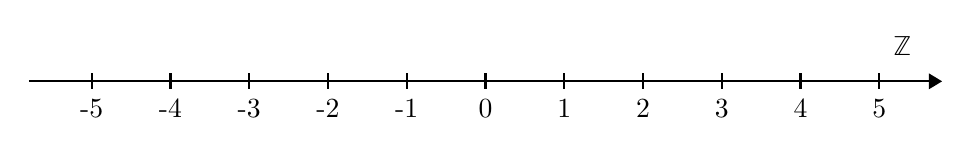
\begin{tikzpicture}
	\draw [-{Triangle}, thick] (-5.8,0) -- (5.8,0);
	\foreach \x in {-5,...,5} {
        \draw[thick](\x,0.1) -- (\x,-0.1);
        \node[below] at (\x,-0.1) {\x};
    }
\node[above] at (5.3,0.2) {$\mathbb{Z}$};
\end{tikzpicture}
\end{document}